\section{Physics}

\begin{Exercise}
Compute the lighting at position $P$ as seen from $E$. Take into account ambient, diffuse and specular lighting.
\begin{center}
  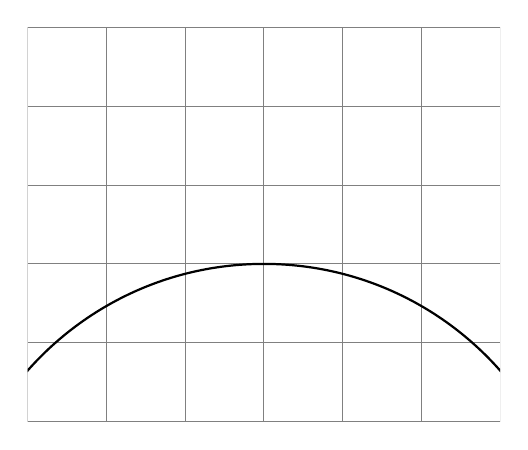
\begin{tikzpicture}
    \path[use as bounding box,clip] (-3,-2) rectangle (3,3);
    \draw[thin,gray] (-5,-5) grid (5,5);
    \coordinate (P) at (0,0);
    \coordinate (L) at (-1,2);
    \coordinate (E) at (2,1);
    \draw[thick] (0,-4) circle (4);
    \point[/point/label=P,/point/position=(P)]
    \point[/point/label=L,/point/position=(L)]
    \point[/point/label=E,/point/position=(E)]
  \end{tikzpicture}
\end{center}
\begin{center}
  \begin{tabular}{lcccc}
    & \textbf{r} & \textbf{g} & \textbf{b} \\
    \toprule
    light source & 1 & 1 & 0 \\
    ambient & 0.2 & 0.2 & 0.2 \\
    diffuse & 0.8 & 0.0 & 0.9 \\
    specular & 0.5 & 0.5 & 0.5 & e = 10
  \end{tabular}
\end{center}
\end{Exercise}


\begin{Exercise}
A sphere is centred at $C(3, 0, 0)$ and has radius $2$.
A ray of light starts at $P(2,2,2)$ and is directed straight towards
the sphere's centre. It hits the sphere at some position $H$.
The ray bounces off the sphere in a mirror-like way and proceeds to hit the YZ-plane at some point $Q$.
\begin{itemize}
  \item What are $H$'s coordinates?
  \item What is the reflected ray's direction?
  \item What are $Q$'s coordinates?
\end{itemize}
\begin{solution}
\[
  \begin{array}{rcl}
    H & = & \displaystyle \left(\frac{7}{3},\frac{4}{3},\frac{4}{3}\right) \\ \\
    N & = & \displaystyle \left(-\frac{1}{3},\frac{2}{3},\frac{2}{3}\right) \\ \\
    R & = & \displaystyle \left(-1,2,2\right) \\ \\
    Q & = & \displaystyle \left(0,6,6\right)
  \end{array}
\]
\end{solution}
\end{Exercise}

\begin{Exercise}
A light ray traverses a piece of glass.
\begin{center}
  \begin{tikzpicture}
    \draw[thick] (0,0) -- ++(0,2);
    \draw[thick] (5,0) -- ++(0,2);
    \draw[light] (-1,2) -- (0,1.5) -- (5,0.5) -- (6,0);

    \draw[|-|,thin] (0,-.5) -- ++(5,0) node[below,midway] {5};
    \draw[dashed,thin] (0,1.5) -- (6,1.5);
    \draw[dashed,thin] (5,0.5) -- (6,0.5);
    \draw[|-|,thin] (6.5,0.5) -- (6.5,1.5) node[right,midway] {x};

    \node at (-2,0) {air};
    \node at (2.5,0) {glass};
    \node at (7,0) {air};
  \end{tikzpicture}
\end{center}
\end{Exercise}
The direction of the light is $(2,-1)$, the thickness of the glass is 5. What is vertical distance travelled by the light ray, represented by $x$?
